% Options for packages loaded elsewhere
\PassOptionsToPackage{unicode}{hyperref}
\PassOptionsToPackage{hyphens}{url}
\documentclass[
  11pt,
]{article}
\usepackage{xcolor}
\usepackage[margin=1in]{geometry}
\usepackage{amsmath,amssymb}
\setcounter{secnumdepth}{5}
\usepackage{iftex}
\ifPDFTeX
  \usepackage[T1]{fontenc}
  \usepackage[utf8]{inputenc}
  \usepackage{textcomp} % provide euro and other symbols
\else % if luatex or xetex
  \usepackage{unicode-math} % this also loads fontspec
  \defaultfontfeatures{Scale=MatchLowercase}
  \defaultfontfeatures[\rmfamily]{Ligatures=TeX,Scale=1}
\fi
\usepackage{lmodern}
\ifPDFTeX\else
  % xetex/luatex font selection
  \setmainfont[]{Verdana}
\fi
% Use upquote if available, for straight quotes in verbatim environments
\IfFileExists{upquote.sty}{\usepackage{upquote}}{}
\IfFileExists{microtype.sty}{% use microtype if available
  \usepackage[]{microtype}
  \UseMicrotypeSet[protrusion]{basicmath} % disable protrusion for tt fonts
}{}
\makeatletter
\@ifundefined{KOMAClassName}{% if non-KOMA class
  \IfFileExists{parskip.sty}{%
    \usepackage{parskip}
  }{% else
    \setlength{\parindent}{0pt}
    \setlength{\parskip}{6pt plus 2pt minus 1pt}}
}{% if KOMA class
  \KOMAoptions{parskip=half}}
\makeatother
\usepackage{color}
\usepackage{fancyvrb}
\newcommand{\VerbBar}{|}
\newcommand{\VERB}{\Verb[commandchars=\\\{\}]}
\DefineVerbatimEnvironment{Highlighting}{Verbatim}{commandchars=\\\{\}}
% Add ',fontsize=\small' for more characters per line
\usepackage{framed}
\definecolor{shadecolor}{RGB}{248,248,248}
\newenvironment{Shaded}{\begin{snugshade}}{\end{snugshade}}
\newcommand{\AlertTok}[1]{\textcolor[rgb]{0.94,0.16,0.16}{#1}}
\newcommand{\AnnotationTok}[1]{\textcolor[rgb]{0.56,0.35,0.01}{\textbf{\textit{#1}}}}
\newcommand{\AttributeTok}[1]{\textcolor[rgb]{0.13,0.29,0.53}{#1}}
\newcommand{\BaseNTok}[1]{\textcolor[rgb]{0.00,0.00,0.81}{#1}}
\newcommand{\BuiltInTok}[1]{#1}
\newcommand{\CharTok}[1]{\textcolor[rgb]{0.31,0.60,0.02}{#1}}
\newcommand{\CommentTok}[1]{\textcolor[rgb]{0.56,0.35,0.01}{\textit{#1}}}
\newcommand{\CommentVarTok}[1]{\textcolor[rgb]{0.56,0.35,0.01}{\textbf{\textit{#1}}}}
\newcommand{\ConstantTok}[1]{\textcolor[rgb]{0.56,0.35,0.01}{#1}}
\newcommand{\ControlFlowTok}[1]{\textcolor[rgb]{0.13,0.29,0.53}{\textbf{#1}}}
\newcommand{\DataTypeTok}[1]{\textcolor[rgb]{0.13,0.29,0.53}{#1}}
\newcommand{\DecValTok}[1]{\textcolor[rgb]{0.00,0.00,0.81}{#1}}
\newcommand{\DocumentationTok}[1]{\textcolor[rgb]{0.56,0.35,0.01}{\textbf{\textit{#1}}}}
\newcommand{\ErrorTok}[1]{\textcolor[rgb]{0.64,0.00,0.00}{\textbf{#1}}}
\newcommand{\ExtensionTok}[1]{#1}
\newcommand{\FloatTok}[1]{\textcolor[rgb]{0.00,0.00,0.81}{#1}}
\newcommand{\FunctionTok}[1]{\textcolor[rgb]{0.13,0.29,0.53}{\textbf{#1}}}
\newcommand{\ImportTok}[1]{#1}
\newcommand{\InformationTok}[1]{\textcolor[rgb]{0.56,0.35,0.01}{\textbf{\textit{#1}}}}
\newcommand{\KeywordTok}[1]{\textcolor[rgb]{0.13,0.29,0.53}{\textbf{#1}}}
\newcommand{\NormalTok}[1]{#1}
\newcommand{\OperatorTok}[1]{\textcolor[rgb]{0.81,0.36,0.00}{\textbf{#1}}}
\newcommand{\OtherTok}[1]{\textcolor[rgb]{0.56,0.35,0.01}{#1}}
\newcommand{\PreprocessorTok}[1]{\textcolor[rgb]{0.56,0.35,0.01}{\textit{#1}}}
\newcommand{\RegionMarkerTok}[1]{#1}
\newcommand{\SpecialCharTok}[1]{\textcolor[rgb]{0.81,0.36,0.00}{\textbf{#1}}}
\newcommand{\SpecialStringTok}[1]{\textcolor[rgb]{0.31,0.60,0.02}{#1}}
\newcommand{\StringTok}[1]{\textcolor[rgb]{0.31,0.60,0.02}{#1}}
\newcommand{\VariableTok}[1]{\textcolor[rgb]{0.00,0.00,0.00}{#1}}
\newcommand{\VerbatimStringTok}[1]{\textcolor[rgb]{0.31,0.60,0.02}{#1}}
\newcommand{\WarningTok}[1]{\textcolor[rgb]{0.56,0.35,0.01}{\textbf{\textit{#1}}}}
\usepackage{graphicx}
\makeatletter
\newsavebox\pandoc@box
\newcommand*\pandocbounded[1]{% scales image to fit in text height/width
  \sbox\pandoc@box{#1}%
  \Gscale@div\@tempa{\textheight}{\dimexpr\ht\pandoc@box+\dp\pandoc@box\relax}%
  \Gscale@div\@tempb{\linewidth}{\wd\pandoc@box}%
  \ifdim\@tempb\p@<\@tempa\p@\let\@tempa\@tempb\fi% select the smaller of both
  \ifdim\@tempa\p@<\p@\scalebox{\@tempa}{\usebox\pandoc@box}%
  \else\usebox{\pandoc@box}%
  \fi%
}
% Set default figure placement to htbp
\def\fps@figure{htbp}
\makeatother
% definitions for citeproc citations
\NewDocumentCommand\citeproctext{}{}
\NewDocumentCommand\citeproc{mm}{%
  \begingroup\def\citeproctext{#2}\cite{#1}\endgroup}
\makeatletter
 % allow citations to break across lines
 \let\@cite@ofmt\@firstofone
 % avoid brackets around text for \cite:
 \def\@biblabel#1{}
 \def\@cite#1#2{{#1\if@tempswa , #2\fi}}
\makeatother
\newlength{\cslhangindent}
\setlength{\cslhangindent}{1.5em}
\newlength{\csllabelwidth}
\setlength{\csllabelwidth}{3em}
\newenvironment{CSLReferences}[2] % #1 hanging-indent, #2 entry-spacing
 {\begin{list}{}{%
  \setlength{\itemindent}{0pt}
  \setlength{\leftmargin}{0pt}
  \setlength{\parsep}{0pt}
  % turn on hanging indent if param 1 is 1
  \ifodd #1
   \setlength{\leftmargin}{\cslhangindent}
   \setlength{\itemindent}{-1\cslhangindent}
  \fi
  % set entry spacing
  \setlength{\itemsep}{#2\baselineskip}}}
 {\end{list}}
\usepackage{calc}
\newcommand{\CSLBlock}[1]{\hfill\break\parbox[t]{\linewidth}{\strut\ignorespaces#1\strut}}
\newcommand{\CSLLeftMargin}[1]{\parbox[t]{\csllabelwidth}{\strut#1\strut}}
\newcommand{\CSLRightInline}[1]{\parbox[t]{\linewidth - \csllabelwidth}{\strut#1\strut}}
\newcommand{\CSLIndent}[1]{\hspace{\cslhangindent}#1}
\setlength{\emergencystretch}{3em} % prevent overfull lines
\providecommand{\tightlist}{%
  \setlength{\itemsep}{0pt}\setlength{\parskip}{0pt}}
\usepackage{float}
\usepackage{graphicx}
\usepackage{geometry}
\usepackage{float}
\floatplacement{figure}{H}
\usepackage{bookmark}
\IfFileExists{xurl.sty}{\usepackage{xurl}}{} % add URL line breaks if available
\urlstyle{same}
\hypersetup{
  hidelinks,
  pdfcreator={LaTeX via pandoc}}

\author{}
\date{\vspace{-2.5em}}

\begin{document}

\begin{titlepage}

    % Logos alineados izquierda y derecha
    \begin{minipage}{0.45\textwidth}
        \raggedright
        
\includegraphics[width=7cm]{data/images/Logo_UNAM.png}
    \end{minipage}
    \hfill
    \begin{minipage}{0.45\textwidth}
        \raggedleft
        
\includegraphics[width=3.4cm]{data/images/Logo_LCG.png}
    \end{minipage}

    \centering
    \vspace*{2cm}

    {\Huge\bfseries Problem Set pt1 \par}
    \vspace{2cm}

    {\Large Genómica Humana \par}
    \vspace{1cm}

    {\Large Jiménez Sotelo Mateo \par}
    \vspace{1cm}

    {\Large Docentes: Dra. Mashaal Sohail, Dra. Araxi Urrutia \par}
    \vspace{1cm}

    {\Large Fecha de entrega: 21 de Abril de 2026 \par}

    \vfill

\end{titlepage}

{
\setcounter{tocdepth}{3}
\tableofcontents
}
\newpage

Fundamento teórico y ejercicios del libro \emph{Population Genetics: A
Concise Guide} (Gillespie (2004))

\section{Genetic Variation}\label{genetic-variation}

\subsection{Problem 1.2}\label{problem-1.2}

\textbf{\emph{Using table 1.2, calculate the frequency of the three
alkaline phosphatase alleles in the English population}}

\begin{quote}
2 points
\end{quote}

\pandocbounded{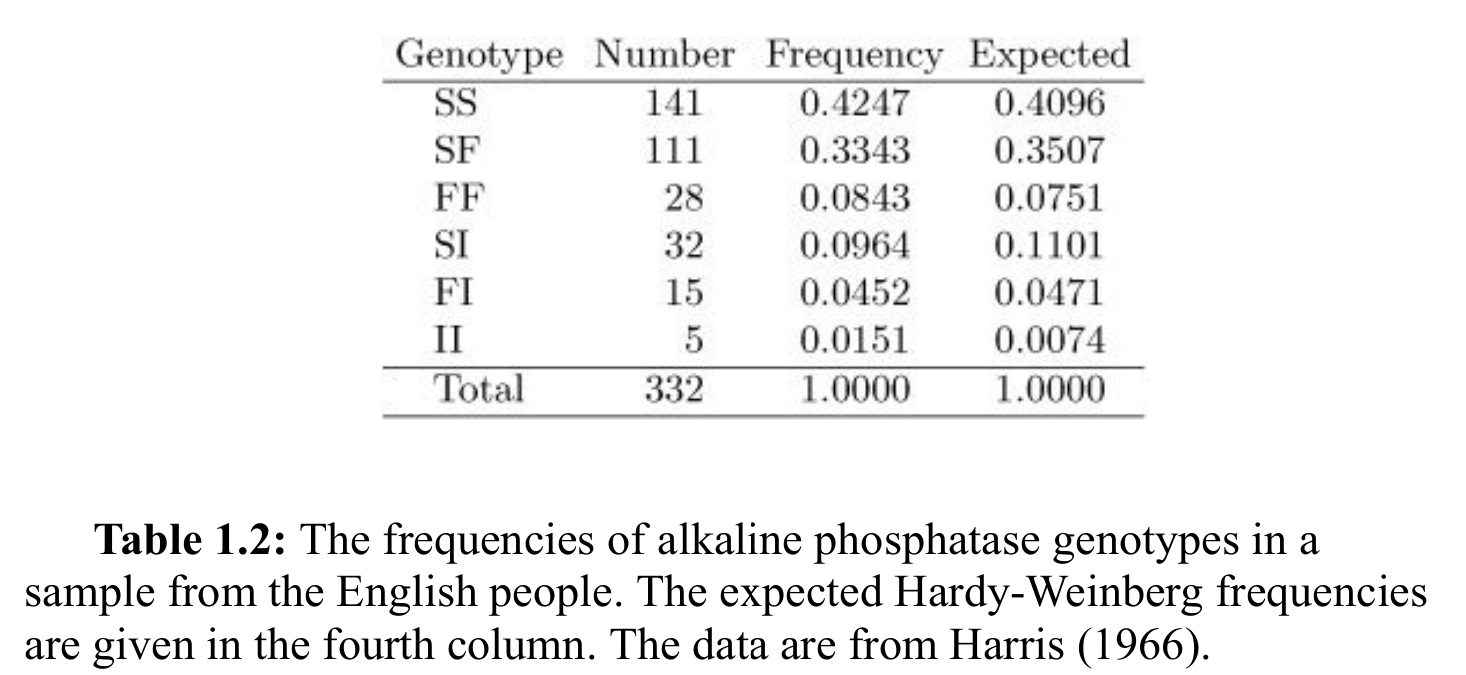
\includegraphics[keepaspectratio]{data/images/gillespie_table_1.2.png}}

La frecuencias de un alelo se logra sumando todas las frecuencias
genotípicas observadas que lo ivolucren, pero dividiendo entre dos las
de heterocigotos (\(f(pq)/2\)) a modo de penalización, porque solo
cuenta con el alelo diana una vez, al contrario del caso homocigoto:

\[
p_A = f(AA) + \frac{1}{2}f(AB) + \frac{1}{2}f(AC)
\]

Dados los alelos \textbf{S}, \textbf{F} e \textbf{I}:

\begin{Shaded}
\begin{Highlighting}[]
\NormalTok{knitr}\SpecialCharTok{::}\NormalTok{opts\_chunk}\SpecialCharTok{$}\FunctionTok{set}\NormalTok{(}
    \AttributeTok{echo =} \ConstantTok{TRUE}\NormalTok{,}
    \AttributeTok{message =} \ConstantTok{FALSE}\NormalTok{,}
    \AttributeTok{warning =} \ConstantTok{FALSE}
\NormalTok{)}

\CommentTok{\# Freqs. genotípicas}
\NormalTok{SS }\OtherTok{\textless{}{-}} \FloatTok{0.4247}
\NormalTok{SF }\OtherTok{\textless{}{-}} \FloatTok{0.3343}
\NormalTok{FF }\OtherTok{\textless{}{-}} \FloatTok{0.0843}
\NormalTok{SI }\OtherTok{\textless{}{-}} \FloatTok{0.0964}
\NormalTok{FI }\OtherTok{\textless{}{-}} \FloatTok{0.0452}
\NormalTok{II }\OtherTok{\textless{}{-}} \FloatTok{0.0151}

\CommentTok{\# Freqs. alélicas}
\NormalTok{S }\OtherTok{\textless{}{-}}\NormalTok{ SS }\SpecialCharTok{+}\NormalTok{ SF}\SpecialCharTok{/}\DecValTok{2} \SpecialCharTok{+}\NormalTok{ SI}\SpecialCharTok{/}\DecValTok{2}
\NormalTok{F }\OtherTok{\textless{}{-}}\NormalTok{ SF}\SpecialCharTok{/}\DecValTok{2} \SpecialCharTok{+}\NormalTok{ FF }\SpecialCharTok{+}\NormalTok{ FI}\SpecialCharTok{/}\DecValTok{2}
\NormalTok{I }\OtherTok{\textless{}{-}}\NormalTok{ SI}\SpecialCharTok{/}\DecValTok{2} \SpecialCharTok{+}\NormalTok{ FI}\SpecialCharTok{/}\DecValTok{2} \SpecialCharTok{+}\NormalTok{ II}
\end{Highlighting}
\end{Shaded}

Así, las frecuencias alélicas de los tres alelos en la población inglesa
son:

\begin{verbatim}
## Frecuencia del alelo S: 0.64
\end{verbatim}

\begin{verbatim}
## Frecuencia del alelo F: 0.274
\end{verbatim}

\begin{verbatim}
## Frecuencia del alelo I: 0.0859
\end{verbatim}

\section{Genetic Drift}\label{genetic-drift}

\subsection{Problem 2.2}\label{problem-2.2}

\textbf{\emph{Write a simulation of genetic drift. Provide your code and
resulting plot}}

\begin{quote}
5 points
\end{quote}

La deriva genética es un proceso estocástico, pudiendo causar
fluctuaciones en las frecuencias alélicas de una población a lo largo
del tiempo, especialmente notorios a medida que la población es más
pequeña. Con base en el libro, se simula este proceso usando el modelo
de \emph{Wright-Fisher}, que cuenta con las siguientes características:

\begin{itemize}
\item
  Población de tamaño constante

  \begin{itemize}
  \tightlist
  \item
    50 individuos diploides
  \end{itemize}
\item
  Generaciones discretas
\item
  Reproducción aleatoria

  \begin{itemize}
  \tightlist
  \item
    \(Ne\) = \(N\)
  \end{itemize}
\item
  Sin mutación
\item
  Sin selección natural
\end{itemize}

La deriva génica se modela directamente con una distribución binomial,
donde el número de éxitos representa el número de alelos \texttt{A} en
la siguiente generación, y la probabilidad de éxito es la
\emph{frecuencia del alelo \texttt{A}} (\texttt{p}) en la generación
pasada. Asimismo, la frecuencia de \texttt{A} se actualiza en cada
generación, dividiendo el número de \texttt{A}s entre el total de
alelos.

\begin{Shaded}
\begin{Highlighting}[]
\FunctionTok{set.seed}\NormalTok{(}\DecValTok{123}\NormalTok{) }\CommentTok{\# Arbitraria, para reproducibilidad}

\CommentTok{\# Parámetros}
\NormalTok{num\_generations }\OtherTok{\textless{}{-}} \DecValTok{100}
\NormalTok{population\_size }\OtherTok{\textless{}{-}} \DecValTok{50}
\NormalTok{num\_simulations }\OtherTok{\textless{}{-}} \DecValTok{5}

\CommentTok{\# Función de simulación}
\NormalTok{simulate\_drift }\OtherTok{\textless{}{-}} \ControlFlowTok{function}\NormalTok{(num\_generations, population\_size) \{}
  \CommentTok{\# Vector en 0s de longitud 100}
\NormalTok{  allele\_freq }\OtherTok{\textless{}{-}} \FunctionTok{numeric}\NormalTok{(num\_generations)}
  \CommentTok{\# Freq. inicial del alelo A}
\NormalTok{  allele\_freq[}\DecValTok{1}\NormalTok{] }\OtherTok{\textless{}{-}} \FloatTok{0.5}

  \CommentTok{\# Simulación}
  \ControlFlowTok{for}\NormalTok{ (gen }\ControlFlowTok{in} \DecValTok{2}\SpecialCharTok{:}\NormalTok{num\_generations) \{ }\CommentTok{\# La 1 es la de la freq. inicial}
    \CommentTok{\# Selección aleatoria de alelos}
    \CommentTok{\# Nuevo num. de A\textquotesingle{}s}
\NormalTok{    alleles }\OtherTok{\textless{}{-}} \FunctionTok{rbinom}\NormalTok{(population\_size, }\DecValTok{2}\NormalTok{, allele\_freq[gen }\SpecialCharTok{{-}} \DecValTok{1}\NormalTok{])}
    \CommentTok{\# Nueva freq. de A}
\NormalTok{    allele\_freq[gen] }\OtherTok{\textless{}{-}} \FunctionTok{sum}\NormalTok{(alleles) }\SpecialCharTok{/}\NormalTok{ (}\DecValTok{2} \SpecialCharTok{*}\NormalTok{ population\_size)}
\NormalTok{  \}}

  \FunctionTok{return}\NormalTok{(allele\_freq)}
\NormalTok{\}}

\CommentTok{\# Plot base {-}{-}\textgreater{} Solo con etiquetas}
\FunctionTok{plot}\NormalTok{(}\ConstantTok{NULL}\NormalTok{,}
  \AttributeTok{xlim =} \FunctionTok{c}\NormalTok{(}\DecValTok{1}\NormalTok{, num\_generations),}
  \AttributeTok{ylim =} \FunctionTok{c}\NormalTok{(}\DecValTok{0}\NormalTok{, }\DecValTok{1}\NormalTok{),}
  \AttributeTok{xlab =} \StringTok{"Generation"}\NormalTok{,}
  \AttributeTok{ylab =} \StringTok{"Allele frequency"}\NormalTok{,}
  \AttributeTok{main =} \StringTok{"Genetic Drift Simulation"}\NormalTok{)}

\CommentTok{\# Distintas simulaciones con seed diferente}
\ControlFlowTok{for}\NormalTok{ (sim }\ControlFlowTok{in} \DecValTok{1}\SpecialCharTok{:}\NormalTok{num\_simulations) \{}
\NormalTok{  freqs }\OtherTok{\textless{}{-}} \FunctionTok{simulate\_drift}\NormalTok{(num\_generations, population\_size)}
  \CommentTok{\# Simulación agregada al plot}
  \FunctionTok{lines}\NormalTok{(}\DecValTok{1}\SpecialCharTok{:}\NormalTok{num\_generations, freqs)}
\NormalTok{\}}
\end{Highlighting}
\end{Shaded}

\pandocbounded{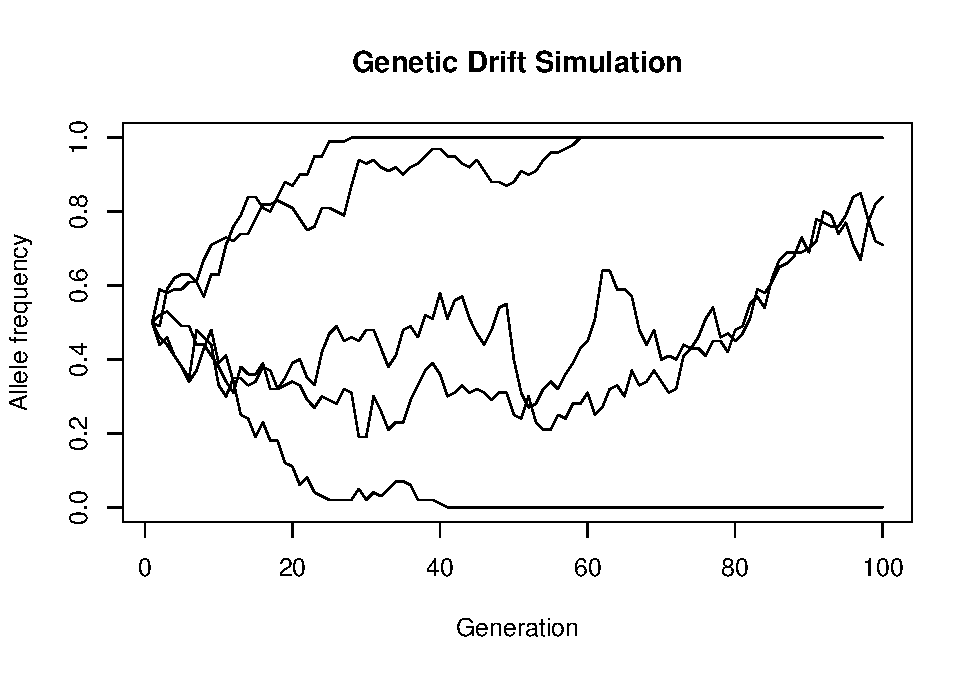
\includegraphics[keepaspectratio]{2_ProblemSet_pt1_JimenezMateo_files/figure-latex/problema 2-1.pdf}}

Observamos que, a lo largo de las generaciones, las frecuencias alélicas
fluctúan de manera aleatoria, ocasionando que en algunos casos el alelo
se fije (\(p_A = 1\)) o, al contrario, se pierda (\(p_A = 0\)).

\subsection{Problem 2.4}\label{problem-2.4}

\textbf{\emph{Graph \(H_t\) and \(G_t\) for 100 generations with
\(H_0 = 1\) and population sizes of \(N=1\), \(10\), \(100\), and
\(1,000,000\)}}

\begin{quote}
5 points
\end{quote}

\begin{itemize}
\tightlist
\item
  \(H_t\): heterocigosidad a través del tiempo
\item
  \(G_t\): homocigosidad a través del tiempo
\end{itemize}

Sabemos que la heterocigosidad se calcula con la siguiente fórmula del
libro:

\[
H_t = H_0 \left(1 - \frac{1}{2N}\right)^t
\]

Así, se grafican los valores de \(H_t\) y \(G_t\) (el complemento de
\(H_t\)) para cada tamaño poblacional:

\begin{quote}
Dado que \(H_0 = 1\), no se incluye en la fórmula
\end{quote}

\begin{Shaded}
\begin{Highlighting}[]
\CommentTok{\# Parámetros}
\NormalTok{num\_generations }\OtherTok{\textless{}{-}} \DecValTok{100}
\NormalTok{t }\OtherTok{\textless{}{-}} \DecValTok{0}\SpecialCharTok{:}\NormalTok{num\_generations}
\NormalTok{population\_sizes }\OtherTok{\textless{}{-}} \FunctionTok{c}\NormalTok{(}\DecValTok{1}\NormalTok{, }\DecValTok{10}\NormalTok{, }\DecValTok{100}\NormalTok{, }\FloatTok{1e6}\NormalTok{)}

\CommentTok{\# Data frame acumulado}
\NormalTok{all\_data }\OtherTok{\textless{}{-}} \FunctionTok{data.frame}\NormalTok{()}

\CommentTok{\# Para cada N}
\ControlFlowTok{for}\NormalTok{ (N }\ControlFlowTok{in}\NormalTok{ population\_sizes) \{}
  \CommentTok{\# Ht {-}{-}\textgreater{} Operación ya vectorizada}
\NormalTok{  H\_t }\OtherTok{\textless{}{-}}\NormalTok{ (}\DecValTok{1} \SpecialCharTok{{-}} \DecValTok{1}\SpecialCharTok{/}\NormalTok{(}\DecValTok{2} \SpecialCharTok{*}\NormalTok{ N))}\SpecialCharTok{\^{}}\NormalTok{t}
  \CommentTok{\# Gt}
\NormalTok{  G\_t }\OtherTok{\textless{}{-}} \DecValTok{1} \SpecialCharTok{{-}}\NormalTok{ H\_t}

  \CommentTok{\# Data frame por N}
\NormalTok{  df }\OtherTok{\textless{}{-}} \FunctionTok{data.frame}\NormalTok{(}
  \AttributeTok{Generation =} \FunctionTok{rep}\NormalTok{(t, }\DecValTok{2}\NormalTok{),}
  \AttributeTok{Value =} \FunctionTok{c}\NormalTok{(H\_t, G\_t),}
  \CommentTok{\# Factor para diferenciar Ht y Gt}
  \AttributeTok{Metric =} \FunctionTok{factor}\NormalTok{(}\FunctionTok{rep}\NormalTok{(}\FunctionTok{c}\NormalTok{(}\StringTok{"Ht"}\NormalTok{, }\StringTok{"Gt"}\NormalTok{), }\AttributeTok{each =} \FunctionTok{length}\NormalTok{(t))),}
  \AttributeTok{N =} \FunctionTok{factor}\NormalTok{(N)}
\NormalTok{  )}

  \CommentTok{\# Acumular data frame}
\NormalTok{  all\_data }\OtherTok{\textless{}{-}} \FunctionTok{rbind}\NormalTok{(all\_data, df)}
\NormalTok{\}}
\end{Highlighting}
\end{Shaded}

\pandocbounded{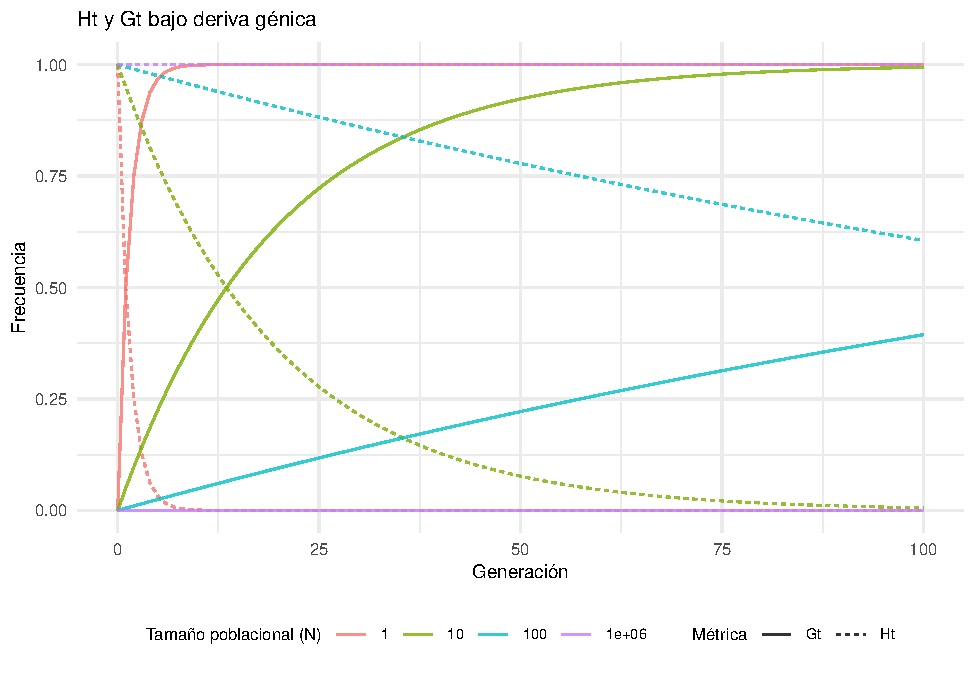
\includegraphics[keepaspectratio]{2_ProblemSet_pt1_JimenezMateo_files/figure-latex/Plot Ht y Gt-1.pdf}}

Se observa la tendencia de la heterocigosidad (\(Ht\)) a disminuir a
medida que pasan las generaciones, especialmente cuando la \(N\) es
pequeña, mientras que la homocigosidad (\(Gt\)) aumenta. En poblaciones
grandes, la tasa de este cambio es mucho más lenta, evidenciando el
efecto de la deriva genética.

\subsection{Problem 2.10}\label{problem-2.10}

\textbf{\emph{If the human generation time is 20 years, what effective
population size for humans is implied by the data?}}

\begin{quote}
2 points
\end{quote}

El libro establece que el tiempo para que la heterocigosidad se reduzca
a la mitad (\(t_{1/2}\)) es \(t_{1/2} \approx 2N_e \ln(2)\). Esto
implica que el tiempo de decaimiento de la variación genética es
proporcional al tamaño efectivo de la población. Podemos despejar
\(N_e\) de la fórmula:

\[
N_e \approx \frac{t_{1/2}}{2 \ln(2)}
\]

Además, se da el ejemplo de una población de tamaño \(N = 10^6\), para
la que se requieren aproximadamente \(1.38 \times 10^6\) generaciones
para reducir la heterocigosidad a la mitad.

Si el tiempo generacional es de 20 años, esto corresponde a
\(1.38 \times 10^6 \times 20 \approx 2.8 \times 10^7\) años, es decir,
\textasciitilde28 millones de años:

\begin{Shaded}
\begin{Highlighting}[]
\NormalTok{generations }\OtherTok{\textless{}{-}} \FloatTok{1.38e6}
\NormalTok{generation\_time }\OtherTok{\textless{}{-}} \DecValTok{20} \CommentTok{\# años}
\NormalTok{time\_years }\OtherTok{\textless{}{-}}\NormalTok{ generations }\SpecialCharTok{*}\NormalTok{ generation\_time}
\NormalTok{time\_years}
\end{Highlighting}
\end{Shaded}

\begin{verbatim}
## [1] 27600000
\end{verbatim}

Sin embargo, en humanos la variación genética observable ha cambiado en
escalas de tiempo evolutivas mucho más cortas (del orden de cientos de
miles de años), y no desde el Oligoceno para acá. Esto implica que el
tiempo de pérdida de heterocigosidad es mucho menor que el del ejemplo
(\(N_e < 10^6\)).

Dado que \(t_{1/2} \propto N_e\) y cambian linealmente, una reducción de
\(n\) órdenes de magnitud en el tiempo implica una reducción similar en
el tamaño efectivo. Asumiendo que la escala de tiempo para humanos es
del orden de \(10^5\) años y recordando que las generaciones son de 20
años, el tiempo en generaciones sería \(10^5 / 20 = 5 \times 10^3\)
generaciones.

Comparando esto con el tiempo para \(N = 10^6\), observamos que
\(\frac{5 \times 10^3}{1.38 \times 10^6} \approx 3.6 \times 10^{-3} \sim 10^{-2}\):

\begin{Shaded}
\begin{Highlighting}[]
\FloatTok{5e3} \SpecialCharTok{/} \FloatTok{1.38e6}
\end{Highlighting}
\end{Shaded}

\begin{verbatim}
## [1] 0.003623188
\end{verbatim}

Esto corresponde aproximadamente a una reducción de dos órdenes de
magnitud. Por lo tanto, el tamaño efectivo de la población humana sería:

\[
N_e \approx (10^6)(10^-2) = 10^4
\]

Este es un ejemplo muy claro de que el tamaño efectivo de la población
humana es mucho menor que su tamaño censal, reflejando la influencia de
la deriva genética en escalas evolutivas.

\section{Natural Selection}\label{natural-selection}

\subsection{Problem 3.1}\label{problem-3.1}

\textbf{\emph{In 1940, the frequency of the medionigra allele in the
Oxford population was about \(p = 0.1\). If the viabilities of the three
genotypes were \(w_{11} = 0.9\), \(w_{12} = 0.95\), and \(w_{22} = 1\),
what would be the frequency of medionigra in the newborns of 1941?}}

\begin{quote}
2 points
\end{quote}

Recordamos la tabla del libro:

\begin{figure}
\centering
\pandocbounded{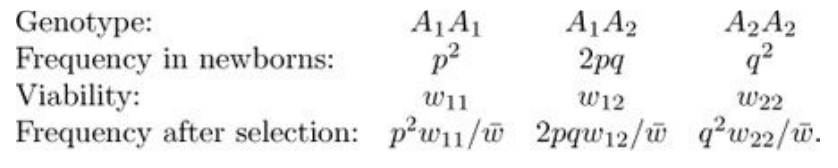
\includegraphics[keepaspectratio]{data/images/gillespie_viability.png}}
\caption{Frecuencia después de selección}
\end{figure}

Sabemos que \(p = 0.1\), por lo que \(q = 1 - p = 0.9\). Además, se nos
dan las viabilidades de los genotipos:

\begin{itemize}
\item
  \(w_{11} = 0.9\) (homocigoto \emph{medionigra})
\item
  \(w_{12} = 0.95\) (heterocigoto)
\item
  \(w_{22} = 1\) (homocigoto alternativo)
\end{itemize}

Así, para encontrar \(p'\)

\[
p' = \frac{p^2 w_{11} + pq w_{12}}{\bar{w}}
\]

donde \(\bar{w}\) es la viabilidad media de la población:

\[
\bar{w} = p^2 w_{11} + 2pq w_{12} + q^2 w_{22}
\]

\begin{Shaded}
\begin{Highlighting}[]
\CommentTok{\# Parámetros}
\NormalTok{p }\OtherTok{\textless{}{-}} \FloatTok{0.1}
\NormalTok{q }\OtherTok{\textless{}{-}} \DecValTok{1} \SpecialCharTok{{-}}\NormalTok{ p}
\NormalTok{w11 }\OtherTok{\textless{}{-}} \FloatTok{0.9}
\NormalTok{w12 }\OtherTok{\textless{}{-}} \FloatTok{0.95}
\NormalTok{w22 }\OtherTok{\textless{}{-}} \DecValTok{1}

\CommentTok{\# Viabilidad media}
\NormalTok{w\_bar }\OtherTok{\textless{}{-}}\NormalTok{ p}\SpecialCharTok{\^{}}\DecValTok{2} \SpecialCharTok{*}\NormalTok{ w11 }\SpecialCharTok{+} \DecValTok{2} \SpecialCharTok{*}\NormalTok{ p }\SpecialCharTok{*}\NormalTok{ q }\SpecialCharTok{*}\NormalTok{ w12 }\SpecialCharTok{+}\NormalTok{ q}\SpecialCharTok{\^{}}\DecValTok{2} \SpecialCharTok{*}\NormalTok{ w22}

\CommentTok{\# Frecuencia después de selección}
\NormalTok{p\_prima }\OtherTok{\textless{}{-}}\NormalTok{ (p}\SpecialCharTok{\^{}}\DecValTok{2} \SpecialCharTok{*}\NormalTok{ w11 }\SpecialCharTok{+}\NormalTok{ p }\SpecialCharTok{*}\NormalTok{ q }\SpecialCharTok{*}\NormalTok{ w12) }\SpecialCharTok{/}\NormalTok{ w\_bar}
\NormalTok{p\_prima}
\end{Highlighting}
\end{Shaded}

\begin{verbatim}
## [1] 0.09545455
\end{verbatim}

\subsection{Problem 3.2}\label{problem-3.2}

\textbf{\emph{If the fitnesses of the genotypes \(A_{1}A_1\),
\(A_{1}A_2\) and \(A_{2}A_2\) are \(w_{11} = 1.5\), \(w_{12} = 1.1\),
and \(w_{22} = 1.0\), respectively, what are the values of the selection
coefficient and the heterozygous effect?}}

\begin{quote}
2 points
\end{quote}

El \emph{fitness} se entiende relativo a un genotipo, en este caso
\(A_{2}A_2\) con \(w_{22} = 1.0\). Dado esto, el \emph{fitness} del
genotipo \(A_{1}A_{1}\), \(w_{11}\), puede entenderse como 1 más el
\textbf{efecto de la selección} (\(s\)). A su vez, el del heterocigoto
(\(A_{1}A_{2}\)), \(w_{12}\), es igualmente 1 más los efectos de la
selección (\(s\)) y de cuánto de eso \emph{permea} en el heterocigoto,
ergo, la \textbf{dominancia} (\(h\)):

\[
w_{12}/w_{22} = 1 + hs \text{, } w_{11}/w_{22} = 1 + s
\]

o, dado que \(w_{22} = 1\), lo que es igual:

\[
w_{12} = 1 + hs \text{, } w_{11} = 1 + s
\]

Despejando, obtenemos que \(s = w_{11} - 1\) y
\(h = \frac{w_{12} - 1}{s}\):

\begin{Shaded}
\begin{Highlighting}[]
\CommentTok{\# Parámetros}
\NormalTok{w11 }\OtherTok{\textless{}{-}} \FloatTok{1.5}
\NormalTok{w12 }\OtherTok{\textless{}{-}} \FloatTok{1.1}
\NormalTok{w22 }\OtherTok{\textless{}{-}} \FloatTok{1.0}
\CommentTok{\# Coeficiente de selección}
\NormalTok{s }\OtherTok{\textless{}{-}}\NormalTok{ w11 }\SpecialCharTok{{-}} \DecValTok{1}
\CommentTok{\# Efecto de la dominancia}
\NormalTok{h }\OtherTok{\textless{}{-}}\NormalTok{ (w12 }\SpecialCharTok{{-}} \DecValTok{1}\NormalTok{) }\SpecialCharTok{/}\NormalTok{ s}
\end{Highlighting}
\end{Shaded}

\begin{verbatim}
## Selection coefficient (s): 0.5
\end{verbatim}

\begin{verbatim}
## Heterozygous effect (h): 0.2
\end{verbatim}

El que \(s\) sea positivo indica que el alelo \(A_1\) es ventajoso (su
\emph{fitness} es mejor que el que confiere \(A_2\)), mientras que el
valor de \(h\) menor a 1 implica que el efecto de la selección en el
heterocigoto es menor que en el homocigoto, es decir, hay una
\textbf{dominancia incompleta} del alelo \(A_1\) sobre \(A_2\).

\subsection{Problem 3.5}\label{problem-3.5}

\textbf{\emph{Write down Equation 3.2 for the special case \(h = 0.5\).
Find the allele frequencies in two successive generations (\(p'\) and
\(p''\)) when the initial value of \(p = 0.1\) and \(s = 0.1\). Continue
this for 200 generations and graph the result}}

\begin{quote}
5 points
\end{quote}

Cuando \(h = 0.5\), tenemos un caso de \textbf{dominancia incompleta}
que nos habla de una \textbf{selección direccional}. La ecuación 3.2 es:

\[
\Delta_{s}p = \frac{pqs[ph + q(1 -h)]}{\bar{w}}
\]

donde \(\bar{w} = 1 - 2pqhs -q^2s\)

A su vez, \({\Delta}_{s}p\) es el cambio en la frecuencia alélica debido
a la selección, por lo que \(p' = p + {\Delta}_{s}p\) y por consiguiente
\(p'' = p' + {\Delta}_{s}p'\).

Escribimos la ecuación particular para \(h = 0.5\):

\[
\Delta_{s}p = \frac{pqs[0.5p +
0.5q]}{\bar{w}} = \frac{pqs[0.5(p + q)]}{\bar{w}} = \frac{pqs[0.5]}{\bar{w}} = \frac{0.5pqs}{\bar{w}}
\]

y planteamos el modelo para \(p\):

\[
p_{t+1} = p_t + \frac{0.5p_t q_t s}{\bar{w}_t}
\]

\begin{Shaded}
\begin{Highlighting}[]
\CommentTok{\# Parámetros}
\NormalTok{s }\OtherTok{\textless{}{-}} \FloatTok{0.1}
\NormalTok{h }\OtherTok{\textless{}{-}} \FloatTok{0.5}
\NormalTok{num\_generations }\OtherTok{\textless{}{-}} \DecValTok{200}
\CommentTok{\# Desde p\_0 hasta p\_200 (Por eso es mejor python :P)}
\NormalTok{p }\OtherTok{\textless{}{-}} \FunctionTok{numeric}\NormalTok{(num\_generations }\SpecialCharTok{+} \DecValTok{1}\NormalTok{)}
\NormalTok{p[}\DecValTok{1}\NormalTok{] }\OtherTok{\textless{}{-}} \FloatTok{0.1}
\NormalTok{q }\OtherTok{\textless{}{-}} \DecValTok{1} \SpecialCharTok{{-}}\NormalTok{ p[}\DecValTok{1}\NormalTok{]}

\CommentTok{\# Apóstrofe de p para imprimir}
\NormalTok{prima }\OtherTok{\textless{}{-}} \StringTok{""}

\ControlFlowTok{for}\NormalTok{ (t }\ControlFlowTok{in} \DecValTok{1}\SpecialCharTok{:}\NormalTok{num\_generations) \{}
  \ControlFlowTok{if}\NormalTok{ (t }\SpecialCharTok{\textless{}=} \DecValTok{3}\NormalTok{) \{}
    \FunctionTok{cat}\NormalTok{(}
        \StringTok{"Generación: "}\NormalTok{, t, }\StringTok{"}\SpecialCharTok{\textbackslash{}t}\StringTok{p"}\NormalTok{, prima, }\StringTok{": "}\NormalTok{,}
        \FunctionTok{round}\NormalTok{(p[t], }\DecValTok{4}\NormalTok{), }\StringTok{"}\SpecialCharTok{\textbackslash{}t}\StringTok{q"}\NormalTok{, prima, }\StringTok{": "}\NormalTok{, }\FunctionTok{round}\NormalTok{(q, }\DecValTok{4}\NormalTok{), }\StringTok{"}\SpecialCharTok{\textbackslash{}n}\StringTok{"}\NormalTok{, }\AttributeTok{sep =} \StringTok{""}
\NormalTok{        )}
\NormalTok{    prima }\OtherTok{\textless{}{-}} \FunctionTok{paste0}\NormalTok{(prima, }\StringTok{"\textquotesingle{}"}\NormalTok{)}
\NormalTok{  \}}
\NormalTok{  q }\OtherTok{\textless{}{-}} \DecValTok{1} \SpecialCharTok{{-}}\NormalTok{ p[t]}
\NormalTok{  mean\_w }\OtherTok{\textless{}{-}} \DecValTok{1} \SpecialCharTok{{-}} \DecValTok{2} \SpecialCharTok{*}\NormalTok{ p[t] }\SpecialCharTok{*}\NormalTok{ q }\SpecialCharTok{*}\NormalTok{ h }\SpecialCharTok{*}\NormalTok{ s }\SpecialCharTok{{-}}\NormalTok{ q}\SpecialCharTok{\^{}}\DecValTok{2} \SpecialCharTok{*}\NormalTok{ s}
\NormalTok{  delta\_p }\OtherTok{\textless{}{-}}\NormalTok{ (}\FloatTok{0.5} \SpecialCharTok{*}\NormalTok{ p[t] }\SpecialCharTok{*}\NormalTok{ q }\SpecialCharTok{*}\NormalTok{ s) }\SpecialCharTok{/}\NormalTok{ mean\_w}
\NormalTok{  p[t }\SpecialCharTok{+} \DecValTok{1}\NormalTok{] }\OtherTok{\textless{}{-}}\NormalTok{ p[t] }\SpecialCharTok{+}\NormalTok{ delta\_p}
\NormalTok{\}}
\end{Highlighting}
\end{Shaded}

\begin{verbatim}
## Generación: 1    p: 0.1  q: 0.9
## Generación: 2    p': 0.1049  q': 0.9
## Generación: 3    p'': 0.1101 q'': 0.8951
\end{verbatim}

\pandocbounded{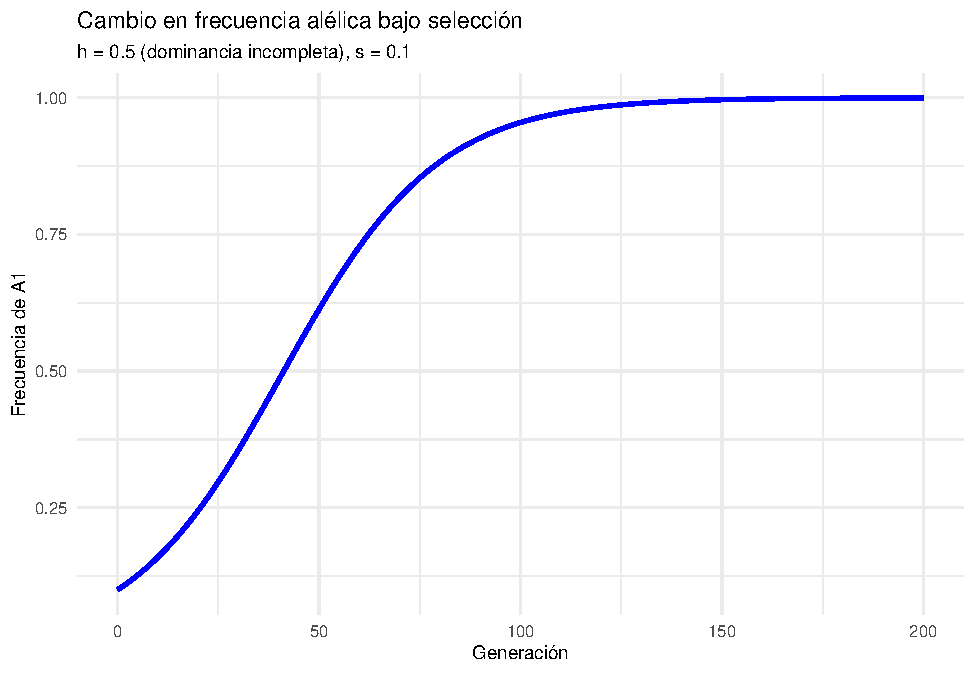
\includegraphics[keepaspectratio]{2_ProblemSet_pt1_JimenezMateo_files/figure-latex/plot problema 7-1.pdf}}

La gráfica describe una forma sigmoide-\emph{like}. Se observa que la
frecuencia alélica aumenta hasta fijarse (\(p = 1\)), con su mayor tasa
de cambio en valores intermedios de \(p\), lo cual es consistente con la
teoría de selección direccional bajo dominancia incompleta.

\subsection{Problem 3.7}\label{problem-3.7}

\textbf{\emph{Graph \({\Delta}_{s}p\) versus \(p\) for an underdominant
locus}}

\begin{quote}
5 points
\end{quote}

Este caso implica selección disruptiva, donde el heterocigoto tiene
menor \emph{fitness} que ambos homocigotos (\(w_{12} < w_{11}\),
\(w_{12} < w_{22}\)).

Para graficar \({\Delta}_{s}p\) contra \(p\) usamos de nueva cuenta:

\[
\Delta_{s}p = \frac{pqs[ph + q(1 -h)]}{\bar{w}}
\]

y la parametrización canónica del libro, relativa a \(w_{11}\):

\[
w_{11} = 1, \quad w_{12} = 1 - hs, \quad w_{22} = 1 - s
\]

lo cual se traduce en un valor de \(h > 1\).

Definiendo arbitrariamente \(s = 0.1\) y \(h = 1.5\), podemos graficar
\({\Delta}_{s}p\) contra \(p\), donde \(0 < p < 1\):

\begin{Shaded}
\begin{Highlighting}[]
\CommentTok{\# Parámetros}
\NormalTok{s }\OtherTok{\textless{}{-}} \FloatTok{0.1}
\NormalTok{h }\OtherTok{\textless{}{-}} \FloatTok{1.5}
\CommentTok{\# p de 0 a 1}
\NormalTok{p }\OtherTok{\textless{}{-}} \FunctionTok{seq}\NormalTok{(}\DecValTok{0}\NormalTok{, }\DecValTok{1}\NormalTok{, }\AttributeTok{length.out =} \DecValTok{100}\NormalTok{)}
\CommentTok{\# q de 1 a 0}
\NormalTok{q }\OtherTok{\textless{}{-}} \DecValTok{1} \SpecialCharTok{{-}}\NormalTok{ p}
\NormalTok{mean\_w }\OtherTok{\textless{}{-}} \DecValTok{1} \SpecialCharTok{{-}} \DecValTok{2} \SpecialCharTok{*}\NormalTok{ p }\SpecialCharTok{*}\NormalTok{ q }\SpecialCharTok{*}\NormalTok{ h }\SpecialCharTok{*}\NormalTok{ s }\SpecialCharTok{{-}}\NormalTok{ q}\SpecialCharTok{\^{}}\DecValTok{2} \SpecialCharTok{*}\NormalTok{ s}
\NormalTok{delta\_p }\OtherTok{\textless{}{-}}\NormalTok{ (p }\SpecialCharTok{*}\NormalTok{ q }\SpecialCharTok{*}\NormalTok{ s }\SpecialCharTok{*}\NormalTok{ (h }\SpecialCharTok{*}\NormalTok{ p }\SpecialCharTok{+}\NormalTok{ q }\SpecialCharTok{*}\NormalTok{ (}\DecValTok{1} \SpecialCharTok{{-}}\NormalTok{ h))) }\SpecialCharTok{/}\NormalTok{ mean\_w}
\end{Highlighting}
\end{Shaded}

\pandocbounded{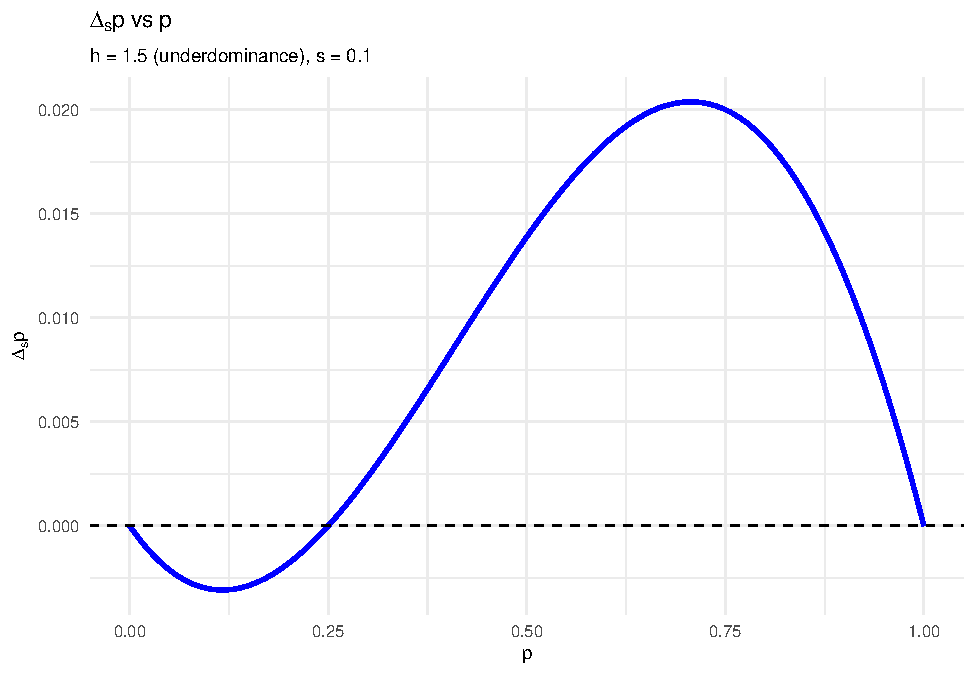
\includegraphics[keepaspectratio]{2_ProblemSet_pt1_JimenezMateo_files/figure-latex/plot problema 8-1.pdf}}

La gráfica muestra que existe un punto intermedio donde
\(\Delta_s p = 0\), el cual corresponde a un equilibrio inestable. Para
valores de \(p\) menores a este punto, \(\Delta_s p < 0\), la frecuencia
alélica tiende a 0, mientras que para valores mayores,
\(\Delta_s p > 0\), la frecuencia tiende a 1.

\section{Linkage Disequilibrium}\label{linkage-disequilibrium}

\subsection{Problem 4.1}\label{problem-4.1}

\textbf{\emph{Derive the three equations for the frequencies of the
\(A1B2\), \(A2B1\), and \(A2B2\) gametes after a round of random
mating}}

\begin{quote}
2 points
\end{quote}

Del libro obtenemos que:

\[
x'_{1} = (1−r)x_{1} + rp_{1}p_{2}
\]

donde \(p_1\) es la frecuencia del alelo \(A_1\) y \(p_2\) la del
\(B_1\), el primer término de lado derecho es la probabilidad de tener
un gameto \(A_1B_1\) sin recombinación, y el segundo es la probabilidad
de obtener este mismo gameto pero por recombinación, a partir de los
alelos \(A_1\) y \(B_1\).

Así, para los gametos \(A_1B_2\), \(A_2B_1\) y \(A_2B_2\),
respectivamente:

\[
x'_{2} = (1−r)x_{2} + rp_{1}(1 - p_{2})
\] \[
x'_{3} = (1−r)x_{3} + r(1 - p_{1})p_{2}
\] \[
x'_{4} = (1−r)x_{4} + r(1 - p_{1})(1- p_{2})
\]

\section{Population subdivision}\label{population-subdivision}

\subsection{Problem 5.1}\label{problem-5.1}

\textbf{\emph{Find \(p\) and \(F\) for a population in which the
genotype frequencies \(A_1A_1\), \(A_1A_2\), and \(A_2A_2\) are
\(0.056\), \(0.288\), and \(0.656\), respectively}}

Recuperamos la tabla del libro:

\begin{figure}
\centering
\pandocbounded{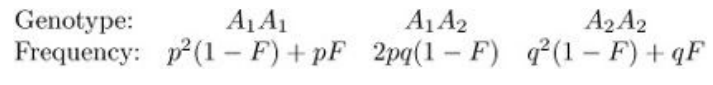
\includegraphics[keepaspectratio]{data/images/gillespie_genotype_freq_nonrand_mating.png}}
\caption{Frecuencia de genotipos con apareamiento no aleatorio}
\end{figure}

\(p\), al igual que antes, es la frecuencia del alelo \(A_1\) y se
calcula con la fórmula:

\[
p = f(A_1A_1) + \frac{1}{2}f(A_1A_2)
\]

lo que nos da \(q = 1 - p\). Por otro lado, \(F\) es el coeficiente de
endogamia, que compara cuánto difiere la heterocigosidad observada de la
esperada por \emph{Hardy-Weinberg}. Dado esto, derivamos del caso
heterocigoto de la tabla:

\[
F = 1 - \frac{f(A_1A_2)}{2pq}
\]

donde \(2pq\) es la heterocigosidad esperada por \emph{Hardy-Weinberg},
\(H_e\), y \(f(A_1A_2)\) la heterocigosidad observada, \(H_o\):

\[
F = 1 - \frac{H_o}{H_e}
\]

Se computan \(p\) y \(F\):

\begin{Shaded}
\begin{Highlighting}[]
\CommentTok{\# Parámetros}
\NormalTok{A11 }\OtherTok{\textless{}{-}} \FloatTok{0.056}
\NormalTok{A12 }\OtherTok{\textless{}{-}} \FloatTok{0.288}

\CommentTok{\# Frecuencia alélica}
\NormalTok{p }\OtherTok{\textless{}{-}}\NormalTok{ A11 }\SpecialCharTok{+}\NormalTok{ A12 }\SpecialCharTok{/} \DecValTok{2}
\NormalTok{q }\OtherTok{\textless{}{-}} \DecValTok{1} \SpecialCharTok{{-}}\NormalTok{ p}

\CommentTok{\# Coeficiente de endogamia}
\NormalTok{F }\OtherTok{\textless{}{-}} \DecValTok{1} \SpecialCharTok{{-}}\NormalTok{ (A12 }\SpecialCharTok{/}\NormalTok{ (}\DecValTok{2} \SpecialCharTok{*}\NormalTok{ p }\SpecialCharTok{*}\NormalTok{ q))}
\end{Highlighting}
\end{Shaded}

\begin{verbatim}
## Frecuencia del alelo A1 (p): 0.2
\end{verbatim}

\begin{verbatim}
## Inbreeding coefficient (F): 0.1
\end{verbatim}

Nótese que no se necesita la frecuencia del genotipo \(A_2A_2\) porque
no involucra al alelo \(A_1\).

\begin{quote}
2 points
\end{quote}

\subsection{Problem 5.10}\label{problem-5.10}

\textbf{\emph{Calculate \(F_{ST}\) for the data in \texttt{Table\ 1.3}.
Pretend that there are only two alleles by using the \(S\) alleles for
\(A_1\) and lumping the other alleles into \(A_2\). First, assume that
all of the subdivisions are the same size (\(c_i = 1/8\)). Next, assume
that}}

\[
c_i =
\begin{cases}
0.2 & i = 1,2,3,4 \\
0.05 & i = 5,6,7,8
\end{cases}
\]

\begin{quote}
3 points
\end{quote}

\begin{figure}
\centering
\pandocbounded{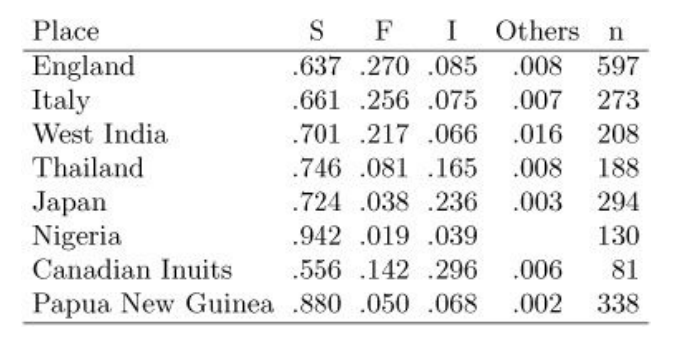
\includegraphics[keepaspectratio]{data/images/gillespie_table1.3.png}}
\caption{Geographic variation in the three alleles of placental alkaline
phosphatase in humans. The ``Others'' category is the total frequency of
alleles other than the three common alleles. The final column is the
sample size. The data are from Roychoudhury and Nei (1988).}
\end{figure}

Se sabe que \(F_{ST} = \frac{H_T - H_S}{H_T}\), donde \(H_T\) es la
heterocigosidad total y \(H_S\) la heterocigosidad promedio dentro de
las subpoblaciones. Para calcular \(H_T\), se necesita la frecuencia
alélica global, que se obtiene haciendo un promedio ponderado de las
frecuencias alélicas de cada subpoblación:

\[
\bar{p} = \sum_{i=1}^{k} c_i p_i
\]

donde \(p_i\) es nuevamente la frecuencia del alelo \(A_1\) (en este
caso, el alelo \(S\)) en la subpoblación \(i\), y \(c_i\) es su peso
relativo.

A partir de esto, la heterocigosidad total se obtiene como la
heterocigosidad esperada bajo \emph{Hardy-Weinberg}, usando la
frecuencia global:

\[
H_T = 2\bar{p}(1 - \bar{p})
\]

Igualmente, la heterocigosidad dentro de cada subpoblación es de nueva
cuenta \(H_i = 2p_i(1 - p_i)\), por lo que la heterocigosidad promedio
dentro de subpoblaciones se vuelve:

\[
H_S = \sum_{i=1}^{k} c_i \, 2p_i(1 - p_i)
\]

\begin{Shaded}
\begin{Highlighting}[]
\CommentTok{\# Frecuencias del alelo S (A1) por subpoblación}
\NormalTok{p }\OtherTok{\textless{}{-}} \FunctionTok{c}\NormalTok{(}
  \AttributeTok{England =} \FloatTok{0.637}\NormalTok{,}
  \AttributeTok{Italy =} \FloatTok{0.661}\NormalTok{,}
  \AttributeTok{West\_India =} \FloatTok{0.701}\NormalTok{,}
  \AttributeTok{Thailand =} \FloatTok{0.746}\NormalTok{,}
  \AttributeTok{Japan =} \FloatTok{0.724}\NormalTok{,}
  \AttributeTok{Nigeria =} \FloatTok{0.942}\NormalTok{,}
  \AttributeTok{Inuit =} \FloatTok{0.556}\NormalTok{,}
  \AttributeTok{Papua\_NG =} \FloatTok{0.880}
\NormalTok{)}

\NormalTok{H\_i }\OtherTok{\textless{}{-}} \DecValTok{2} \SpecialCharTok{*}\NormalTok{ p }\SpecialCharTok{*}\NormalTok{ (}\DecValTok{1} \SpecialCharTok{{-}}\NormalTok{ p)}

\CommentTok{\# Caso 1 {-}{-}\textgreater{} c\_i = 1/8}
\NormalTok{c\_equal }\OtherTok{\textless{}{-}} \FunctionTok{rep}\NormalTok{(}\DecValTok{1}\SpecialCharTok{/}\DecValTok{8}\NormalTok{, }\FunctionTok{length}\NormalTok{(p))}
\CommentTok{\# Freq global}
\NormalTok{glob\_p }\OtherTok{\textless{}{-}} \FunctionTok{sum}\NormalTok{(c\_equal }\SpecialCharTok{*}\NormalTok{ p)}
\CommentTok{\# Heterocigosidad total}
\NormalTok{H\_T\_equal }\OtherTok{\textless{}{-}} \DecValTok{2} \SpecialCharTok{*}\NormalTok{ glob\_p }\SpecialCharTok{*}\NormalTok{ (}\DecValTok{1} \SpecialCharTok{{-}}\NormalTok{ glob\_p)}
\CommentTok{\# Heterocigosidad promedio}
\NormalTok{H\_S\_equal }\OtherTok{\textless{}{-}} \FunctionTok{sum}\NormalTok{(c\_equal }\SpecialCharTok{*}\NormalTok{ H\_i)}
\CommentTok{\# Fst}
\NormalTok{F\_ST\_equal }\OtherTok{\textless{}{-}}\NormalTok{ (H\_T\_equal }\SpecialCharTok{{-}}\NormalTok{ H\_S\_equal) }\SpecialCharTok{/}\NormalTok{ H\_T\_equal}


\CommentTok{\# Caso 2 {-}{-}\textgreater{} pesos desiguales}
\CommentTok{\# 4 subpoblaciones con cada peso}
\NormalTok{c\_weighted }\OtherTok{\textless{}{-}} \FunctionTok{c}\NormalTok{(}\FloatTok{0.2}\NormalTok{, }\FloatTok{0.2}\NormalTok{, }\FloatTok{0.2}\NormalTok{, }\FloatTok{0.2}\NormalTok{, }\FloatTok{0.05}\NormalTok{, }\FloatTok{0.05}\NormalTok{, }\FloatTok{0.05}\NormalTok{, }\FloatTok{0.05}\NormalTok{)}
\CommentTok{\# Freq. global}
\NormalTok{p\_bar\_weighted }\OtherTok{\textless{}{-}} \FunctionTok{sum}\NormalTok{(c\_weighted }\SpecialCharTok{*}\NormalTok{ p)}
\CommentTok{\# Heterocigosidad total}
\NormalTok{H\_T\_weighted }\OtherTok{\textless{}{-}} \DecValTok{2} \SpecialCharTok{*}\NormalTok{ p\_bar\_weighted }\SpecialCharTok{*}\NormalTok{ (}\DecValTok{1} \SpecialCharTok{{-}}\NormalTok{ p\_bar\_weighted)}
\CommentTok{\# Heterocigosidad promedio}
\NormalTok{H\_S\_weighted }\OtherTok{\textless{}{-}} \FunctionTok{sum}\NormalTok{(c\_weighted }\SpecialCharTok{*}\NormalTok{ H\_i)}
\CommentTok{\# Fst}
\NormalTok{F\_ST\_weighted }\OtherTok{\textless{}{-}}\NormalTok{ (H\_T\_weighted }\SpecialCharTok{{-}}\NormalTok{ H\_S\_weighted) }\SpecialCharTok{/}\NormalTok{ H\_T\_weighted}
\end{Highlighting}
\end{Shaded}

\begin{verbatim}
## Caso 1 (c_i = 1/8):
\end{verbatim}

\begin{verbatim}
## p⁻ = 0.7309
\end{verbatim}

\begin{verbatim}
## H_T = 0.3934
\end{verbatim}

\begin{verbatim}
## H_S = 0.3653
\end{verbatim}

\begin{verbatim}
## F_ST = 0.0713
\end{verbatim}

\begin{verbatim}
## Caso 2 (pesos desiguales):
\end{verbatim}

\begin{verbatim}
## p⁻ = 0.7041
\end{verbatim}

\begin{verbatim}
## H_T = 0.4167
\end{verbatim}

\begin{verbatim}
## H_S = 0.4024
\end{verbatim}

\begin{verbatim}
## F_ST = 0.0342
\end{verbatim}

Vemos que el valor de \(F_{ST}\) es sustancialmente más alto en el caso
de un solo peso, debido a que, al ponderar más fuertemente a ciertas
subpoblaciones, se modifican tanto la frecuencia alélica global como la
heterocigosidad promedio dentro de poblaciones.

Se observa que, al asignar menor peso a poblaciones con frecuencias
alélicas más extremas (como Nigeria), la heterogeneidad entre
subpoblaciones disminuye, y eso se refleja en un \(F_{ST}\) menor,
mostrando que \(F_{ST}\) no es propio del sistema, sino que depende de
cómo se ponderen las subpoblaciones.

\emph{Does the fact that \(F_{ST}\) depends on your assumption about the
\(c_i\) make you nervous?}

Si bien esto podría parecer preocupante, en realidad refleja que
\(F_{ST}\) describe la estructura genética relativa a un esquema de
muestreo o a la definición de la población total. Es decir, el valor de
\(F_{ST}\) depende de cómo se ponderan las subpoblaciones, pero esto
\textbf{no} cambia la forma en que la variación genética está
distribuida, sino cómo se resume.

\section{Quantitative Genetics}\label{quantitative-genetics}

\subsection{Problem 6.4}\label{problem-6.4}

The following measurements of weights are from a single parent and its
offspring and are expressed as deviations from the mean. What is the
heritability of this trait?

\[
(-0.002, -0.391),\ (1.566, 1.747),\ (0.542, -2.127),\ (-0.285, -1.623),\ (-1.519, -0.876),
\]

\[
(-1.136, -0.705),\ (0.907, 0.458),\ (0.435, -0.287),\ (1.292, 0.153),\ (-0.640, 0.711)
\]

\textbf{(2 points)}

\begin{figure}
\centering
\pandocbounded{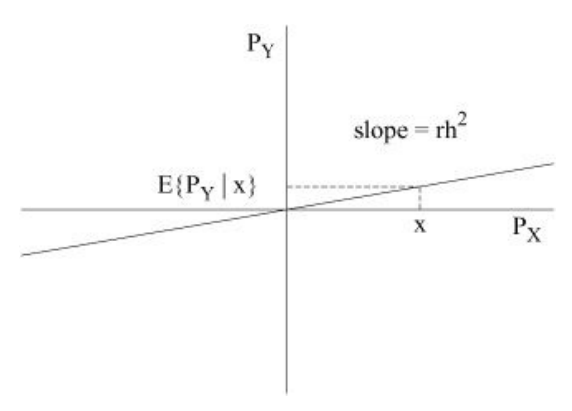
\includegraphics[keepaspectratio]{data/images/gillespie_fig_5.3.png}}
\caption{The use of regression to find the expected value of the
phenotype of relative Y given that the phenotype of relative X is x.}
\end{figure}

La heredabilidad (\(h^2\)) puede estimarse como la \textbf{pendiente de
la regresión} de los valores del descendiente entre los del progenitor.
Esto equivale a:

\[
h^2 = \beta = \frac{\text{Cov}(P_X,P_Y)}{\text{Var}(P_X)} = rh^2
\]

donde \(X\) representa el valor del progenitor y \(Y\) el del
descendiente.

\begin{Shaded}
\begin{Highlighting}[]
\CommentTok{\# Parent y offspring dados}
\NormalTok{data }\OtherTok{\textless{}{-}} \FunctionTok{matrix}\NormalTok{(}\FunctionTok{c}\NormalTok{(}
  \SpecialCharTok{{-}}\FloatTok{0.002}\NormalTok{, }\SpecialCharTok{{-}}\FloatTok{0.391}\NormalTok{,}
   \FloatTok{1.566}\NormalTok{,  }\FloatTok{1.747}\NormalTok{,}
   \FloatTok{0.542}\NormalTok{, }\SpecialCharTok{{-}}\FloatTok{2.127}\NormalTok{,}
  \SpecialCharTok{{-}}\FloatTok{0.285}\NormalTok{, }\SpecialCharTok{{-}}\FloatTok{1.623}\NormalTok{,}
  \SpecialCharTok{{-}}\FloatTok{1.519}\NormalTok{, }\SpecialCharTok{{-}}\FloatTok{0.876}\NormalTok{,}
  \SpecialCharTok{{-}}\FloatTok{1.136}\NormalTok{, }\SpecialCharTok{{-}}\FloatTok{0.705}\NormalTok{,}
   \FloatTok{0.907}\NormalTok{,  }\FloatTok{0.458}\NormalTok{,}
   \FloatTok{0.435}\NormalTok{, }\SpecialCharTok{{-}}\FloatTok{0.287}\NormalTok{,}
   \FloatTok{1.292}\NormalTok{,  }\FloatTok{0.153}\NormalTok{,}
  \SpecialCharTok{{-}}\FloatTok{0.640}\NormalTok{,  }\FloatTok{0.711}
\NormalTok{), }\AttributeTok{ncol =} \DecValTok{2}\NormalTok{, }\AttributeTok{byrow =} \ConstantTok{TRUE}\NormalTok{)}

\CommentTok{\# Separar variables}
\NormalTok{parent }\OtherTok{\textless{}{-}}\NormalTok{ data[,}\DecValTok{1}\NormalTok{] }\CommentTok{\# Col 1}
\NormalTok{offspring }\OtherTok{\textless{}{-}}\NormalTok{ data[,}\DecValTok{2}\NormalTok{] }\CommentTok{\# Col 2}

\CommentTok{\# Correlación}
\NormalTok{r }\OtherTok{\textless{}{-}} \FunctionTok{cor}\NormalTok{(parent, offspring)}

\CommentTok{\# R\^{}2 para evaluar regresión}
\NormalTok{R2 }\OtherTok{\textless{}{-}}\NormalTok{ r}\SpecialCharTok{\^{}}\DecValTok{2}

\CommentTok{\# Heredabilidad}
\NormalTok{h2 }\OtherTok{\textless{}{-}} \FunctionTok{cov}\NormalTok{(parent, offspring) }\SpecialCharTok{/} \FunctionTok{var}\NormalTok{(parent)}
\end{Highlighting}
\end{Shaded}

\begin{verbatim}
## h^2 = 0.4852
\end{verbatim}

\begin{verbatim}
## R^2 = 0.1907
\end{verbatim}

\pandocbounded{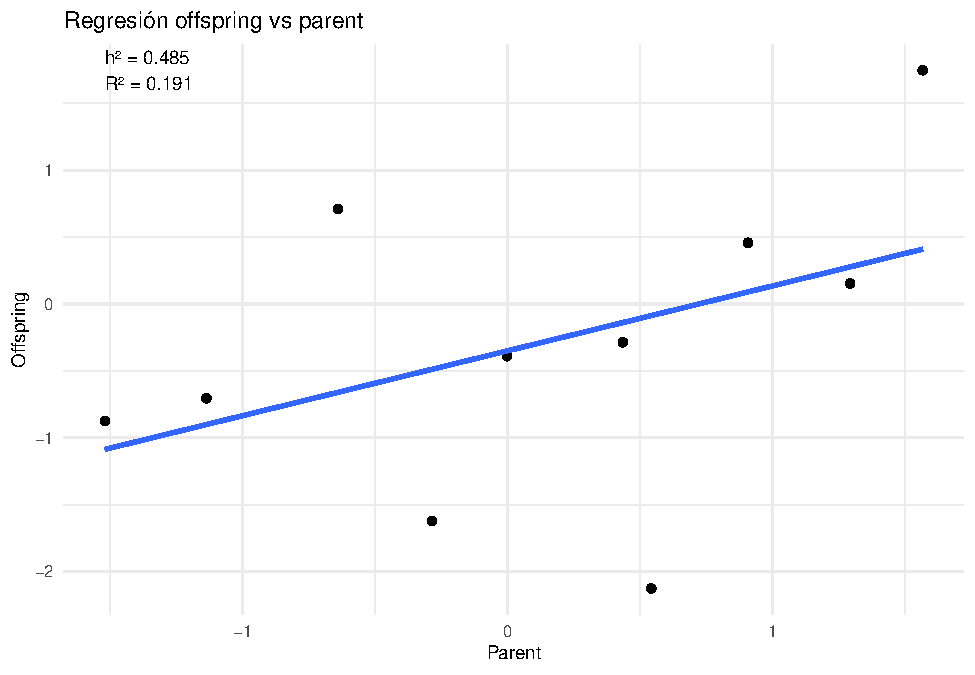
\includegraphics[keepaspectratio]{2_ProblemSet_pt1_JimenezMateo_files/figure-latex/plot problema 11-1.pdf}}

El valor de \(h^2 \approx 0.485\) indica una heredabilidad media, por lo
que una parte importante de la variación fenotípica se debe a efectos
genéticos aditivos.

Sin embargo, el valor relativamente bajo de \(R^2 \approx 0.191\) indica
que la relación lineal entre progenitor y descendiente es algo débil,
con una alta dispersión de los datos alrededor de la recta de regresión.
Esto sugiere que, además de los efectos genéticos, existe una
contribución considerable de factores ambientales (\(\epsilon\)).

Así, vemos que aunque el rasgo tiene una base genética observable, la
predicción del fenotipo del descendiente solo a partir del progenitor es
limitada.

\section*{Referencias}\label{referencias}
\addcontentsline{toc}{section}{Referencias}

\phantomsection\label{refs}
\begin{CSLReferences}{1}{0}
\bibitem[\citeproctext]{ref-gillespie2004}
Gillespie, John H. 2004. \emph{Population Genetics: A Concise Guide}.
2nd ed. Baltimore: Johns Hopkins University Press.

\end{CSLReferences}

\end{document}
